\documentclass{standalone}
\usepackage{tikz}
\usetikzlibrary{calc,intersections,through}

\begin{document}

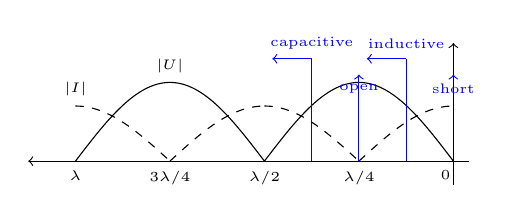
\begin{tikzpicture}
    \draw[<-]  (-2.4,0) -- (3.2,0);
    \draw[->]  (3,-0.3) -- (3,1.5);

    \draw (-1.8,0) sin (-0.6,1);
    \draw (-0.6,1) cos (0.6,0);
    \draw (0.6,0) sin (1.8,1);
    \draw (1.8,1) cos (3,0);

    \draw[dashed] (-1.8,0.7) cos (-0.6,0);
    \draw[dashed] (-0.6,0) sin (0.6,0.7);
    \draw[dashed] (0.6,0.7) cos (1.8,0);
    \draw[dashed] (1.8,0) sin (3,0.7);

    \draw (-1.8,0)node [below,font=\tiny,] {$\lambda$};
    \draw (-0.6,0)node [below,font=\tiny,] {$3\lambda/4$};
    \draw (0.6,0)node [below,font=\tiny,] {$\lambda/2$};
    \draw (1.8,0)node [below,font=\tiny,] {$\lambda/4$};
    \draw (2.9,0)node [below,font=\tiny,] {$0$};

    \draw[->,blue] (3,1.1)node[anchor=north,font=\tiny] {short};
    \draw[blue] (2.4,0) -- (2.4,1.3);
    \draw[->,blue] (2.4,1.3)node[anchor=south,font=\tiny] {inductive} -- (1.9,1.3);
    \draw[->,blue] (1.8,0) -- (1.8,1.1)node[anchor=north,font=\tiny] {open};
    \draw[blue] (1.2,0) -- (1.2,1.3);
    \draw[->,blue] (1.2,1.3)node[anchor=south,font=\tiny] {capacitive} -- (0.7,1.3);

    \draw(-0.6,1)node[above,font=\tiny]{$|U|$};
    \draw(-1.8,0.7)node[above,font=\tiny]{$|I|$};

\end{tikzpicture}

\end{document}